\documentclass[presentation]{beamer}

\usepackage[utf8]{inputenc}
% \usepackage[T1]{fontenc}
\usepackage{fixltx2e}
\usepackage{graphicx}
% \usepackage{longtable}
% \usepackage{tabu}
\usepackage{makecell}
\usepackage{float}
\usepackage{subcaption}
\usepackage{wrapfig}
\usepackage{rotating}
\usepackage[normalem]{ulem}
\usepackage{amsmath}
% \usepackage{textcomp}
% \usepackage{marvosym}
% \usepackage{wasysym}
% \usepackage{amssymb}
\usepackage{hyperref}
\usepackage{ragged2e}
\usepackage{xcolor}


\usepackage{bm}

\usepackage{amsmath,amssymb}
\newcommand{\bx}{\mathbf{x}}
\newcommand{\bv}{\mathbf{v}}
\newcommand{\bp}{\mathbf{p}}
\newcommand{\bq}{\mathbf{q}}
\newcommand{\by}{\mathbf{y}}

\newcommand{\bbR}{\mathbb{R}}
\newcommand{\bbN}{\mathbb{N}}

\newcommand{\bxi}{\bm{\xi}}
\newcommand{\bal}{\bm{\alpha}}
\newcommand{\bth}{\bm{\theta}}

\usepackage{etoolbox}
\let\bbordermatrix\bordermatrix
\patchcmd{\bbordermatrix}{8.75}{4.75}{}{}
\patchcmd{\bbordermatrix}{\left(}{\left[}{}{}
\patchcmd{\bbordermatrix}{\right)}{\right]}{}{}

\usepackage[authoryear, round]{natbib}

\newcommand{\sidebysidecaption}[4]{%
\RaggedRight%
  \begin{minipage}[t]{#1}
    \vspace*{0pt}
    #3
  \end{minipage}
  \hfill%
  \begin{minipage}[t]{#2}
    \vspace*{0pt}
    #4
\end{minipage}%
}

%% colors
\definecolor{Red}{rgb}{0.7,0,0}
\definecolor{Blue}{rgb}{0,0,0.8}
\definecolor{Green}{rgb}{0,0.8,0}
\definecolor{Gray}{rgb}{0.8,0.8,0.8}
\definecolor{Orange}{rgb}{1,.65,0}

\usepackage{hyperref}
\hypersetup{
  hyperindex = {true},
  colorlinks = {true},
  linktocpage = {true},
  plainpages = {false},
  linkcolor = {Blue},
  citecolor = {Blue},
  urlcolor = {Red},
  pdfstartview = {Fit},
  pdfpagemode = {UseOutlines},
  pdfview = {XYZ null null null},
  pdfkeywords={proteomics, spatial, dynamics, integration, regulation, computational biology},
  pdfsubject={Research talk},
  pdfcreator={Laurent Gatto}}

%% knitr

%% maxwidth is the original width if it is less than linewidth
%% otherwise use linewidth (to make sure the graphics do not exceed the margin)
\makeatletter
\def\maxwidth{ %
  \ifdim\Gin@nat@width>\linewidth
    \linewidth
  \else
    \Gin@nat@width
  \fi
}
\makeatother

\definecolor{fgcolor}{rgb}{0.345, 0.345, 0.345}
\newcommand{\hlnum}[1]{\textcolor[rgb]{0.686,0.059,0.569}{#1}}%
\newcommand{\hlstr}[1]{\textcolor[rgb]{0.192,0.494,0.8}{#1}}%
\newcommand{\hlcom}[1]{\textcolor[rgb]{0.678,0.584,0.686}{\textit{#1}}}%
\newcommand{\hlopt}[1]{\textcolor[rgb]{0,0,0}{#1}}%
\newcommand{\hlstd}[1]{\textcolor[rgb]{0.345,0.345,0.345}{#1}}%
\newcommand{\hlkwa}[1]{\textcolor[rgb]{0.161,0.373,0.58}{\textbf{#1}}}%
\newcommand{\hlkwb}[1]{\textcolor[rgb]{0.69,0.353,0.396}{#1}}%
\newcommand{\hlkwc}[1]{\textcolor[rgb]{0.333,0.667,0.333}{#1}}%
\newcommand{\hlkwd}[1]{\textcolor[rgb]{0.737,0.353,0.396}{\textbf{#1}}}%

\usepackage{framed}
\makeatletter
\newenvironment{kframe}{%
 \def\at@end@of@kframe{}%
 \ifinner\ifhmode%
  \def\at@end@of@kframe{\end{minipage}}%
  \begin{minipage}{\columnwidth}%
 \fi\fi%
 \def\FrameCommand##1{\hskip\@totalleftmargin \hskip-\fboxsep
 \colorbox{shadecolor}{##1}\hskip-\fboxsep
     % There is no \\@totalrightmargin, so:
     \hskip-\linewidth \hskip-\@totalleftmargin \hskip\columnwidth}%
 \MakeFramed {\advance\hsize-\width
   \@totalleftmargin\z@ \linewidth\hsize
   \@setminipage}}%
 {\par\unskip\endMakeFramed%
 \at@end@of@kframe}
\makeatother

\definecolor{shadecolor}{rgb}{.97, .97, .97}
\definecolor{messagecolor}{rgb}{0, 0, 0}
\definecolor{warningcolor}{rgb}{1, 0, 1}

\definecolor{errorcolor}{rgb}{1, 0, 0}
\newenvironment{knitrout}{}{} % an empty environment to be redefined in TeX

\usepackage{alltt}
\usepackage[utf8]{inputenc}
\usepackage[T1]{fontenc}
\usepackage{fixltx2e}
\usepackage{graphicx}
\usepackage{longtable}
\usepackage{float}
\usepackage{wrapfig}
\usepackage{rotating}
\usepackage[normalem]{ulem}
\usepackage{amsmath}
\usepackage{textcomp}
\usepackage{marvosym}
\usepackage{wasysym}
\usepackage{amssymb}


\date{29 March 2019 -- ISBA}

\title{Probabilistic modelling of protein sub-cellular localisation}

\author{Laurent Gatto\\
  \url{laurent.gatto@uclouvain.be}\\
  de Duve Institute -- UCLouvain
  \bigskip
  slides \url{http://bit.ly/20190329ISBA}
}


% \AtBeginSection[] % Do nothing for \section*
% {
%   \begin{frame}<beamer>
%     \frametitle{Plan}
%     \tableofcontents[currentsection]
%   \end{frame}
% }


\begin{document}

\maketitle

% \begin{frame}{}
%   Who?
% \end{frame}

\begin{frame}{Abstract}
  In biology, \textbf{localisation is function} - understanding the
  sub-cellular localisation of proteins is paramount to comprehend the
  context of their functions. Mass spectrometry-based \textbf{spatial
    proteomics} and contemporary \textbf{machine learning} enable to
  build proteome-wide spatial maps, informing us on the location of
  thousands of proteins. Nevertheless, while some proteins can be
  found in a single location within a cell, up to half of proteins may
  reside in multiple locations, can dynamically re-localise, or reside
  within an unknown functional compartment, leading to considerable
  \textbf{uncertainty} in associating a protein to their sub-cellular
  location. Recent advances enable us to \textbf{probabilistically}
  model protein localisation as well as quantify the uncertainty in
  the location assignments, thus leading to better and more
  trustworthy biological interpretation of the data.
\end{frame}


\begin{frame}
  \begin{block}{}
  \begin{enumerate}
  \item \textbf{Use case}: spatial proteomics.
  \item Novel \textbf{computational biology research and developments}
    to acquire reliable biological knowledge.
  \item \textbf{Behind the scenes}: software/data structures and open research
    practice.
  \end{enumerate}
  \end{block}
\end{frame}


\section{Spatial proteomics}

\begin{frame}{}
  \begin{center}
    \Large{\textbf{Use case}: spatial proteomics.}
  \end{center}
\end{frame}

\subsection*{The LOPIT pipeline}

\label{sec:spintro}

%% \begin{frame}{Regulations}
%%   \begin{figure}[h]
%%     \centering
%%     \includegraphics[width=1\linewidth]{Figures2/regulation.jpg}
%%   \end{figure}
%% \end{frame}

\label{sec:spspatprot}

\begin{frame}{Cell organisation - regulation of protein localisation}
  \begin{center}
    \includegraphics[width=1\linewidth]{figs_all/Animal_cell_structure.png} \\
    \textbf{\textcolor{Blue}{Spatial proteomics}} is the systematic
    study of protein localisations.
  \end{center}

  \tiny Image from Wikipedia
  \url{http://en.wikipedia.org/wiki/Cell_(biology)}.
\end{frame}

% \begin{frame}{Spatial proteomics - Why?}
%   \begin{itemize}
%   \item Localisation is function
%   \item Mis-localisation \citep{Kau2004,Laurila2009}
%   \item Re-localisation
%   \end{itemize}
% \end{frame}

\begin{frame}{Spatial proteomics - Why?}
  \begin{block}{Localisation is function}
    \begin{itemize}
    \item The cellular sub-division allows cells to establish a range
      of distinct micro-environments, each favouring different
      biochemical reactions and interactions and, therefore, allowing
      each compartment to fulfil a particular functional role.
    \item Localisation and sequestration of proteins within
      sub-cellular niches is a fundamental mechanism for the
      post-translational regulation of protein function.
    \end{itemize}
  \end{block}
  \begin{block}{Re-localisation in}
    \begin{itemize}
    \item \textcolor{Blue}{Differentiation} stem cells.
    \item \textcolor{Blue}{Activation} of biological processes.
    \end{itemize}
    %% Examples later.
  \end{block}
\end{frame}

\begin{frame}{Spatial proteomics - Why?}
  \begin{block}{Mis-localisation}
    Disruption of the targeting/trafficking process alters proper
    sub-cellular localisation, which in turn perturb the cellular
    functions of the proteins.
    \begin{itemize}
    \item Abnormal protein localisation leading to the \textbf{loss of
        functional} effects in diseases \citep{Laurila2009}.
    \item Disruption of the nuclear/cytoplasmic transport (nuclear
      pores) have been detected in many types of \textbf{carcinoma
        cells} \citep{Kau2004}.
    \item Sub-cellular localisation of MC4R with ADCY3 at neuronal
      primary cilia underlies a common pathway for genetic
      predisposition to \textbf{obesity} \citep{Siljee:2018}.
    \end{itemize}
  \end{block}

\end{frame}


\subsubsection*{Experimental designs}
\label{sec:expdesign}

\begin{frame}{Spatial proteomics - How, experimentally}
  \begin{figure}
    \includegraphics[width=.8\linewidth]{figs_all/F02-expdesigns.pdf}
    \caption{Organelle proteomics approaches \citep{Gatto:2010}}
  \end{figure}
\end{frame}

\begin{frame}{Fusion proteins and immunofluorescence}

  \begin{figure}[h]
    \centering
    \includegraphics[width=.35\linewidth]{figs_all/Localisations02eng.jpg}
    \includegraphics[width=.45\linewidth]{figs_all/if_selected.jpg}
    \caption{Targeted protein localisation. Example of discrepancies
      between IF and FPs as well as between FP tagging at the N and C
      termini \citep{Stadler:2013}.}
  \end{figure}
\end{frame}


\subsubsection*{Gradient approaches}
\label{sec:grad}

\begin{frame}{Spatial proteomics - How, experimentally}
  \begin{figure}
    \includegraphics[width=.8\linewidth]{figs_all/F02-expdesigns.pdf}
    \caption{Organelle proteomics approaches
      \citep{Gatto:2010}.}
  \end{figure}

  \textbf{Gradient approaches}: \cite{Dunkley:2006},
  \cite{Foster2006}.

  \bigskip

  \textbf{Explorative/discovery approaches},
  \textcolor{Blue}{steady-state \textbf{global localisation maps}}.
\end{frame}


\begin{frame}{}
  \begin{figure}
    % \includegraphics[width=.8\linewidth]{figs_all/F03-protocols-8plex.pdf}
    % \includegraphics[width=.5\linewidth]{figs_all/expdesign.pdf}
    \includegraphics[width=.39\linewidth]{figs_all/workflow_primary.pdf}
  \end{figure}
\end{frame}

\subsubsection*{The data}
\label{sec:data}

\begin{frame}{Quantitation data}
  \begin{center}
    \begin{tabular}{|l|llll|}
      \hline
      & Fraction$_{\text{1}}$ & Fraction$_{\text{2}}$ & \ldots{} & Fraction$_{\text{L}}$ \\
      \hline
      {\bf x}$_{\text{1}}$ & $x_{\text{1,1}}$ & $x_{\text{1,2}}$ & \ldots{} & $x_{\text{1,L}}$ \\
      {\bf x}$_{\text{2}}$ & $x_{\text{2,1}}$ & $x_{\text{2,2}}$ & \ldots{} & $x_{\text{2,L}}$ \\
      {\bf x}$_{\text{3}}$ & $x_{\text{3,1}}$ & $x_{\text{3,2}}$ & \ldots{} & $x_{\text{3,L}}$ \\
      \vdots & \vdots & \vdots & \vdots & \vdots \\
      {\bf x}$_{\text{i}}$ & $x_{\text{i,1}}$ & $x_{\text{i,2}}$ & \ldots{} & $x_{\text{i,L}}$ \\
      \vdots & \vdots & \vdots & \vdots & \vdots \\
      {\bf x}$_{\text{N}}$ & $x_{\text{N,1}}$ & $x_{\text{N,2}}$ & \ldots{} & $x_{\text{N, L}}$ \\
      \hline
    \end{tabular}
  \end{center}
\end{frame}

\begin{frame}{Quantitation data and organelle markers}
  \begin{center}
    \begin{tabular}{|l|llll||l|}
      \hline
      & Fraction$_{\text{1}}$ & Fraction$_{\text{2}}$ & \ldots{} & Fraction$_{\text{L}}$ & markers\\
      \hline
      {\bf x}$_{\text{1}}$ & $x_{\text{1,1}}$ & $x_{\text{1,2}}$ & \ldots{} & $x_{\text{1,L}}$ & unknown \\
      {\bf x}$_{\text{2}}$ & $x_{\text{2,1}}$ & $x_{\text{2,2}}$ & \ldots{} & $x_{\text{2,L}}$ & \textcolor{Red}{$loc_{1}$}\\
      {\bf x}$_{\text{3}}$ & $x_{\text{3,1}}$ & $x_{\text{3,2}}$ & \ldots{} & $x_{\text{3,L}}$ & unknown \\
      \vdots & \vdots & \vdots & \vdots & \vdots & \vdots \\
      {\bf x}$_{\text{i}}$ & $x_{\text{i,1}}$ & $x_{\text{i,2}}$ & \ldots{} & $x_{\text{i,L}}$ & \textcolor{Blue}{$loc_{k}$}\\
      \vdots & \vdots & \vdots & \vdots & \vdots & \vdots\\
      {\bf x}$_{\text{N}}$ & $x_{\text{N,1}}$ & $x_{\text{N,2}}$ & \ldots{} & $x_{\text{N, K}}$ & unknown \\
      \hline
    \end{tabular}
  \end{center}
\end{frame}

\begin{frame}{}
  \begin{center}
    \Large{Data analysis}
  \end{center}
\end{frame}


\subsection*{Data analysis}
\label{sec:comp}


\begin{frame}{Data analysis}
  \begin{itemize}
  \item \textbf{Visualisation} (cluster, unsupervised learning)
  \item \textbf{Classification} (supervised learning)
  \item \textbf{Novelty detection} (semi-supervised learning)
  \item Data integration (transfer learning)
  \item \textbf{Multi-localisation (Bayesian spatial proteomics)}
  \item Spatial dynamics
  \end{itemize}
  \centering

  \bigskip

  {\Large To uncover and understand biology}
\end{frame}



\subsubsection*{Visualisation}
\label{sec:viz}

\begin{frame}{Visualisation}
  \begin{figure}
    \centering
    \includegraphics[width=.6\linewidth]{figs_all/F04-analyses.pdf}
    \caption{From \cite{Gatto:2010}, \textit{Arabidopsis thaliana} data
      from \cite{Dunkley:2006}}
  \end{figure}
\end{frame}

\subsubsection*{Machine learning}
\label{sec:ml}

\begin{frame}{Supervised Machine Learning}
  \begin{figure}[h]
    \centering
    \includegraphics[width=\linewidth]{figs_all/hyperlopit-class.pdf}
    \caption{Support vector machines classifier (after 5\% FDR
      classification cutoff) on the embryonic stem cell data from
      \cite{Christoforou:2016}.}
  \end{figure}
\end{frame}

\section{Computational biology}

\begin{frame}{}
  \begin{center}
    \Large{Novel \textbf{computational biology research and developments}
    to acquire reliable biological knowledge.}
  \end{center}
\end{frame}

\subsection{Novelty detection}

\begin{frame}{Importance of annotation}

  \begin{columns}[t]
    \begin{column}[T]{0.43\textwidth}
      \begin{centering}
        \includegraphics[width=1\linewidth]{figs_all/tan2009r1org.pdf}
      \end{centering}
    \end{column}
    \begin{column}[T]{0.56\textwidth}
      \includegraphics[width=1\linewidth]{figs_all/Animal_cell_structure.png}
    \end{column}
  \end{columns}
  Incomplete annotation, and therefore lack of training data, for
  many/most organelles. \textit{Drosophila} data from \cite{Tan2009}.
\end{frame}

\begin{frame}{Semi-supervised learning: novelty detection}
  \begin{figure}
    \includegraphics[width=.48\linewidth]{figs_all/tan2009r1org.pdf}
    \includegraphics[width=.5\linewidth]{figs_all/pdres2fig.pdf}
    \caption{Left: Original \textit{Drosophila} data from
      \cite{Tan2009}. Right: After semi-supervised learning and
      classification, \cite{Breckels:2013}.}
  \end{figure}
\end{frame}

\begin{frame}{}
  \begin{figure}
    \includegraphics[width=.48\linewidth]{figs_more/phenodisco.pdf}
    \caption{The effect of organelle discovery upon sub-cellular protein
      localisation \cite{Breckels:2013}.}
  \end{figure}
\end{frame}

% \begin{frame}
%   \centering
%   \begin{columns}[t]
%     \begin{column}[T]{0.4\textwidth}
%       \begin{figure}[h]
%         \includegraphics[width=.9\linewidth]{figs_all/tan2009r1org.pdf} \\
%         \includegraphics[width=.9\linewidth]{figs_all/pdres2fig.pdf}
%       \end{figure}
%     \end{column}
%     \begin{column}[T]{0.59\textwidth}
%       \begin{figure}[h]
%         \includegraphics[width=.9\linewidth]{figs_all/phenodisco.pdf}
%       \end{figure}
%     \end{column}
%   \end{columns}
%   % \caption{The \texttt{phenoDisco} algorithm \citep{Breckels:2013}.}
% \end{frame}

%% \subsection{Improving on LOPIT}

%% \begin{frame}{Improving on LOPIT}

%%   Improving is obtaining better \textbf{sub-cellular resolution} to
%%   increase the number of protein that can be \textbf{confidently}
%%   assigned to a sub-cellular niche $\Rightarrow$ \textbf{biological
%%     discoveries}.

%%   \begin{figure}[h]
%%     \centering
%%     \includegraphics[width=1\linewidth]{./figs_all/E14-lopit-hyperlopit.pdf}
%%     \caption{E14TG2a embryonic stem cells: old (left, published in
%%       \cite{Breckels:2013}) \textit{vs.} new, better resolved (right)
%%       experiments (\cite{Christoforou:2016}).}
%%   \end{figure}

%% \end{frame}

%% \begin{frame}{Improving on LOPIT}


%%   \centering
%%   \begin{tabular}{| p{5cm} | p{5cm} |}
%%     \hline
%%     \makecell{LOPIT\\ \cite{Dunkley:2006} \\ \cite{Gatto:2014}}    & \makecell{\textbf{Computational}:\\ \textit{transfer learning}\\ \cite{Breckels:2016}} \\
%%     \hline
%%     \makecell{\textbf{Experimental}:\\ \textit{hyperLOPIT}\\ \cite{Christoforou:2016} \\ \cite{Mulvey:2017} \\ \cite{Breckels:2016b}} & \makecell{\textbf{Biological}\\\textbf{discoveries}}  \\
%%     \hline
%%   \end{tabular}
%% \end{frame}

%% \subsubsection{Experimental advances: hyperLOPIT }

%% \begin{frame}{Experimental advances: hyperLOPIT \cite{Christoforou:2016}}
%%   \begin{figure}[h]
%%     \centering
%%     \includegraphics[width=.7\linewidth]{./figs_all/nprot-hyperlopit-2017-026-F1.jpg}
%%     \caption{From \cite{Mulvey:2017} \textit{Using \textbf{hyperLOPIT}
%%         to perform high-resolution mapping of the spatial proteome}:
%%       (1) organelle separation and enrichment by \textbf{density
%%         gradient ultracentrifugation}, (2) \textbf{chromatin and
%%         cytosol} enrichment fractions, and (3) accurate quantification
%%       using \textbf{synchronous precursor selection (SPS)-MS$^3$ for
%%         TMT 11-plex} quantification.}
%%     \label{fig:hyperlopit}
%%   \end{figure}
%% \end{frame}

%% \begin{frame}
%%   \begin{figure}[h]
%%     \centering
%%     \includegraphics[width=1\linewidth]{./figs_all/E14-lopit-hyperlopit-rep1.pdf}
%%     \caption{E14TG2a LOPIT on 8 fractions (using iTRAQ 8-plex) and
%%       1109 proteins \textit{vs.}  hyperLOPIT on 10 fractions (using
%%       TMT 11-plex) and SPS-MS$^3$ for 5032 proteins.}
%%   \end{figure}

%% \end{frame}

\subsection{Computational advances: Transfer learning}

\begin{frame}{Computational advances: Transfer learning}
  What about using \textbf{addition data}, such as annotations from
  the Gene Ontology (GO), sequence features (pseudo aminoacid
  composition), signal peptide, trans-membrane domains (length,
  number, ...), images (IF, FP), interaction data, prediction
  software, \ldots

  \begin{block}{}
    \begin{itemize}
    \item From a \underline{user perspective}: \textbf{"free/cheap"}
      vs. expensive and time-consuming experiments.
    \item Abundant (all proteins, 100s of features) vs. (experimentally)
      limited/\textbf{targeted} (1000s of proteins, 6 -- 20 of features)
    \item For localisation in \underline{system at hand}: \textit{low}
      vs. high \textbf{quality}
    \item \textbf{Static} vs. \textbf{dynamic}
    \end{itemize}
  \end{block}

\end{frame}

\begin{frame}{}

  \begin{block}{Transfer learning}
    Support/complement the \textbf{primary} target domain
    (experimental data) with \textbf{auxiliary} data (annotation,
    imaging, PPI, ...)  features without compromising the integrity of
    our primary data.
  \end{block}

\end{frame}


\begin{frame}
  \begin{center}
    \includegraphics[width=.7\linewidth]{figs_all/workflow.pdf}
  \end{center}
\end{frame}


\begin{frame}{Transfer learning results}

  \begin{figure}[h]
    \centering
    \includegraphics[width=.8\linewidth]{./figs_all/2016-PLoSCB-TL-classifierDiscriminationPowerk5.pdf}
    \caption{{\footnotesize From \cite{Breckels:2016} \textit{Learning from
          heterogeneous data sources: an application in spatial
          proteomics}.}
    }
\label{fig:tlres}
  \end{figure}

\end{frame}

\subsection{Embracing uncertainty}

\begin{frame}{How much do we learn? How much do we miss?}
  \begin{figure}
    \includegraphics[width=.8\linewidth]{./figs_all/preConcludePlot.png}
  \end{figure}
\end{frame}

\begin{frame}{}
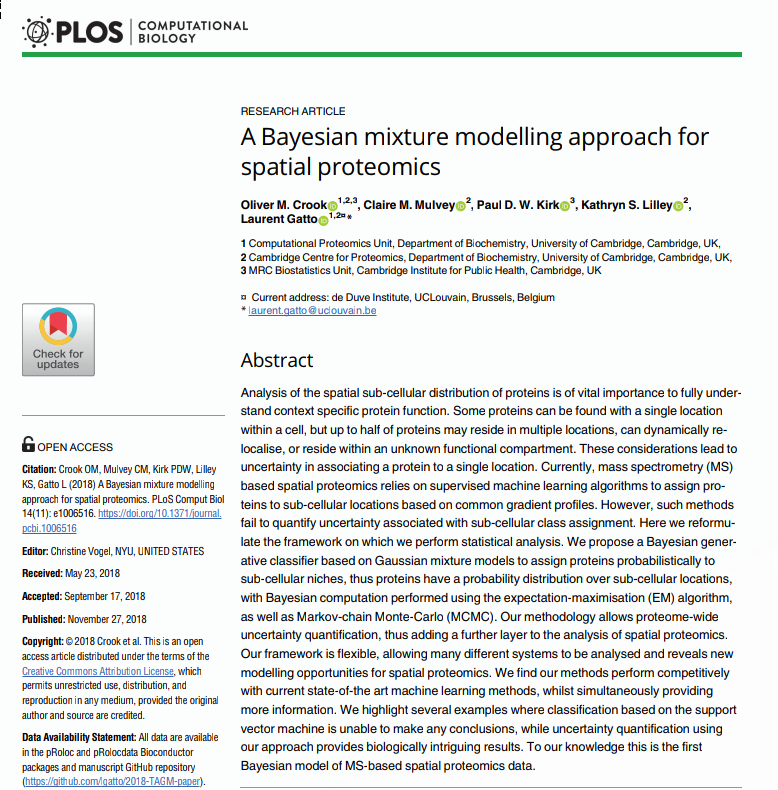
\includegraphics[width=1\linewidth]{./figs_more/plostagm.png}
\end{frame}


\begin{frame}{A Bayesian Mixture Modelling Approach For Spatial Proteomics}

  \begin{itemize}

    \item<+-> \textit{T Augmented Gaussian Mixture model (TAGM)} is a
      \textbf{multivariate Gaussian generative model} for MS-based
      spatial proteomics data. It posits that each annotated
      sub-cellular niche can be modelled by a multivariate Gaussian
      distribution.

    \item<+-> With the prior knowledge that many proteins are not
      captured by known sub-cellular niches, we augment our model with
      an \textbf{outlier component}. Outliers are often dispersed and
      thus this additional component is described by a heavy-tailed
      distribution: the multivariate Student's t-distribution, leading
      us to a \textit{T Augmented Gaussian Mixture model}.

    \item<+-> This methodology allows proteome-wide
      \textbf{uncertainty quantification}, thus adding a further layer
      to the analysis of spatial proteomics.

  \end{itemize}
\end{frame}


\begin{frame}{}

    We initially model the distribution of profiles associated with
    proteins that localise to the $k$-th component as multivariate
    normal with mean vector $\boldsymbol{\mu}_k$ and covariance matrix
    $\Sigma_k$, so that:

    \begin{align}
      {\bf x}_i | z_i = k \quad \sim \mathcal{N}(\boldsymbol{\mu}_k, \Sigma_k) \label{equation::preq}
    \end{align}

    \pause

    We extend it by introducing an additional \textit{outlier
      component}. To do this, we augment our model by introducing a
    further indicator latent variable $\phi$. Each protein ${\bf x}_i$
    is now described by an additional variable $\phi_i$, with $\phi_i
    = 1$ indicating that protein ${\bf x}_i$ belongs to a organelle
    derived component and $\phi_i = 0$ indicating that protein ${\bf
      x}_i$ is not well described by these known components. This
    outlier component is modelled as a multivariate T distribution
    with degrees of freedom $\kappa$, mean vector $\bf{M}$, and scale
    matrix $V$.

    \begin{align}
      {\bf x}_i | z_i = k, \phi_i \quad \sim \mathcal{N}(\boldsymbol{\mu}_k, \Sigma_k)^{\phi_i}\mathcal{T}(\kappa, \boldsymbol{M}, V)^{1 - \phi_i }
    \end{align}


\end{frame}

\begin{frame}{}
  \begin{figure}
    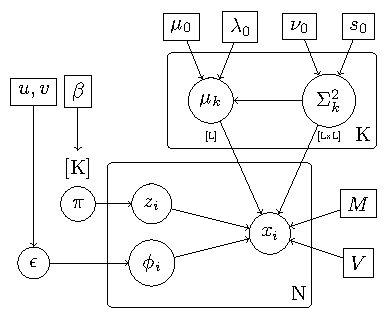
\includegraphics[width=1\linewidth]{./figs_more/graphmodel2.pdf}
    \caption{Plate diagram specifying the conditional independencies
      and parameters in TAGM.}
  \end{figure}
\end{frame}


\begin{frame}[fragile]{}
      \begin{figure}
        \sidebysidecaption{0.65\linewidth}{0.3\linewidth}{
          \includegraphics[width=1\linewidth]{./figs_all/pca12-ellipses-1.pdf}
        }{
          \caption{\scriptsize \justifying Illustration of how the
            TAGM model describes the pluripotent mouse embryonic stem
            cell data. Each ellipse contains a proportion of total
            probability of a particular multivariate Gaussian density.
            The outer ellipse contains $99\%$ of the total probability
            whilst the middle and inner ellipses contain $95\%$ and
            $90\%$ of the probability respectively.}
          \label{fig:tagm}
        }
      \end{figure}

      %% NOTE that while some sub-cellular clusters overlap along PC1 and
      %% PC2, they are separated along additional dimensions.

\end{frame}

\begin{frame}{}
      \begin{figure}
        \includegraphics[width=1\linewidth]{./figs_all/tagm_pca_res.pdf}
        \caption{Assignment of proteins of
          \textit{unknown} location to one of the annotated
          classes. The dots are scaled according to the protein
          assignment probabilities.}
      \end{figure}
\end{frame}

\begin{frame}{}
  \begin{figure}
    \includegraphics[width=.8\linewidth]{./figs_all/ConcludePlot.pdf}
  \end{figure}
\end{frame}

\begin{frame}
  \begin{figure}
    \centering
    \sidebysidecaption{0.55\linewidth}{0.42\linewidth}{
      \includegraphics[width=1\linewidth]{./figs_all/Q924C1-prob-1.pdf}
    }{
    \caption{\scriptsize \justifying Exportin 5 (Q924C1) forms part of
      the micro-RNA export machinery, transporting miRNA from the
      nucleus to the cytoplasm for further processing.  It then
      translocates back through the nuclear pore complex to return to
      the nucleus to mediate further transport between nucleus and
      cytoplasm. The model correctly infers that it most likely
      localises to the cytosol but there is some uncertainty with this
      assignment. This uncertainty is reflected in possible assignment
      of Exportin 5 to the nucleus non-chromatin and reflects the
      multi-location of the protein.}  }
    %% NOTE SVM failed to classify exportin 5 to any of the two
    %% biologically plausible locations, arguably due to the similarity
    %% of the cytosol and peroxysome, to which it got assigned.

  \end{figure}
\end{frame}


\begin{frame}{Whole sub-cellular proteome uncertainty}
  \begin{figure}
    \centering
    \includegraphics[width=.32\linewidth]{./figs_all/pca-tagm-mcmc-1.pdf}
    \includegraphics[width=.32\linewidth]{./figs_all/pca-tagm-map-1.pdf}
    \includegraphics[width=.32\linewidth]{./figs_all/prob-vs-shannon-1.pdf}
  \end{figure}
\end{frame}



%% \subsubsection{Dual-localisation}

%% \begin{frame}
%%   \textcolor{Blue}{\textbf{Dual-localisation}} Proteins may be present
%%   simultaneously in several organelles (e.g. trafficking). Simulation
%%   on \textit{A. thaliana} data from \cite{Dunkley:2006}
%%   \citep{Gatto:2014a} (left). Example from embryonic stem cells
%%   \citep{Christoforou:2016} (right).
%%   \begin{columns}
%%     \begin{column}{.5\textwidth}
%%       \includegraphics[width=1\linewidth]{figs_all/dual-loc.pdf}<+->
%%     \end{column}
%%     \begin{column}{.5\textwidth}<+->
%%       \centering
%%       \includegraphics[width=.8\linewidth]{figs_all/Tfe3.png}\\
%%       \tiny From \cite{Betschinger:2013} \\
%%       \includegraphics[width=1\linewidth]{figs_all/Tfe3.pdf}
%%     \end{column}
%%   \end{columns}
%% \end{frame}

\subsection{Spatial dynamics}

\begin{frame}{Spatial dynamics}
  \begin{block}{Trans-localisation event during monocyte to macrophage
      differentiation}
    Investigate the effect of lipopolysaccharides (LPS)-mediated
    inflammatory response in human monocytic cells (THP-1)
  \end{block}

  \begin{block}{Data}
    \begin{itemize}
    \item Triplicate \textbf{temporal} profiling (0, 2, 4, 6, 12, 24
      hours).
    \item Triplicate \textbf{spatial} profiling (0 vs 12 hours) -
      early trafficking, before actual morphological differentiation
      at 24h.
    \end{itemize}
  \end{block}

  Work lead by \textbf{Dr Claire Mulvey} at the Cambridge Centre for
  Proteomics.

\end{frame}



\begin{frame}
  \begin{figure}[h]
    \centering
    \includegraphics[width=\linewidth]{./figs_all/lps.pdf}
    \caption{Spatial maps of unstimulated and LPS-treated cells
      (combined triplicates).}
  \end{figure}
\end{frame}

\begin{frame}
  \begin{figure}[h]
    \centering
    \includegraphics[width=\linewidth]{./figs_all/lps-pkc.pdf}
    \caption{Relocation of Protein Kinase C $\alpha$ and $\beta$ from the
      cytosol to the plasma membrane, \textbf{driving maturation into
        a differentiated macrophage phenotype}.}
  \end{figure}
\end{frame}

\begin{frame}
  \begin{figure}[h]
    \centering
    \includegraphics[width=\linewidth]{./figs_all/lps-stat.pdf}
    \caption{Relocation of Signal transducer and activator of
      transcription 6 (STAT6) from the cytosol to the Nucleus,
      \textbf{activating anti-bacterial and anti-viral-like
        response}. Validated by microscopy and see also
      \cite{Chen:2011}.}
  \end{figure}
\end{frame}


\section{Computational infrastructure}

\begin{frame}{}
  \begin{center}
    \Large{\textbf{Behind the scenes}: software/data structures and
      open research practice.}
  \end{center}
\end{frame}


\begin{frame}{}

  Beyond the figures\footnote{... which are all reproducible, by the way.}

  \begin{itemize}
  \item<+-> Software: \textbf{infrastructure}
    (\href{http://bioconductor.org/packages/MSnbase}{\texttt{MSnbase}},
    \cite{Gatto:2012}), \textbf{dedicated machine learning}
    (\href{http://bioconductor.org/packages/pRoloc}{\texttt{pRoloc}},
    \cite{Gatto:2014a}), \textbf{interactive
      visualisation}\footnote{\url{https://lgatto.shinyapps.io/christoforou2015/}}
    (\href{http://bioconductor.org/packages/pRolocGUI}{\texttt{pRolocGUI}},
    \cite{pRolocGUI}) and \textbf{data}
    (\href{http://bioconductor.org/packages/pRolocdata}{\texttt{pRolocdata}},
    \cite{Gatto:2014a}) for spatial proteomics.
  \item<+-> The \href{http://bioconductor.org/}{\textbf{Bioconductor}}
    \citep{Huber:2015} ecosystem for high throughput biology data
    analysis and comprehension: \textbf{open source}, and
    \textbf{coordinated and collaborative\footnote{between and within
        domains/software} open development}, enabling
    \textbf{reproducible research}, enables understanding of the data
    (not a black box) and \textbf{drive scientific innovation}.
  \end{itemize}
\end{frame}


%% \begin{frame}
%%   \begin{figure}[h]
%%     \centering
%%     \includegraphics[width=.8\linewidth]{./figs_all/g.png}
%%     \caption{\textbf{Collaboration between packages}: Dependency graph
%%       containing 41 MS and proteomics-tagged packages (out of 100+)
%%       and their dependencies. }
%%   \end{figure}
%% \end{frame}

%% \begin{frame}{\textbf{MSnbase} example}

%%   \begin{figure}[h]
%%     \centering
%%     \includegraphics[width=.8\linewidth]{./figs_all/msnbase-contributors-2.png}
%%     \caption{\textbf{Collaboration within packages}: Contributions to the
%%       \texttt{MSnbase} package (1220 downloads from unique IP
%%       addresses in January 2018) since its creation, the last one
%%       leading to \textbf{common proteomics/metabolomics
%%         infrastructure}. More details:
%%       \url{https://lgatto.github.io/msnbase-contribs/}}
%%     \label{fig:msnbase}
%%   \end{figure}

%% \end{frame}

\begin{frame}{Open research: open source software}
  \centering
  \begin{figure}
  \includegraphics[width=\linewidth]{./figs_all/pRoloc_screen.png}
    \caption{\cite{Gatto:2014} Left: Public repository for the \texttt{pRoloc} software
      (\url{https://github.com/lgatto/pRoloc}). Right: offical
      Bioconductor page.}
  \end{figure}
\end{frame}

\begin{frame}{Open and reproducible research}
  \centering
  \begin{figure}
    \includegraphics[width=1\linewidth]{./figs_all/qsep_screen.png}
    \caption{\cite{Gatto:2018} reproducible document
      (\url{https://github.com/lgatto/QSep-manuscript}), preprint
      (\url{https://doi.org/10.1101/377630}) and paper
      (\url{https://doi.org/10.1016/j.cbpa.2018.11.015}).}
  \end{figure}
\end{frame}

\begin{frame}{}
Working with open and reproducible research in mind doesn't mean
releasing everything prematurely, it means

\begin{itemize}
\item managing research in a way one can find data and results at
  every stage

\item one can reproduce results, re-run/compare them with new data or
  different methods/parameters, and

\item  one can release data (or parts thereof) when/if appropriate.
\end{itemize}
\end{frame}

%% \begin{frame}{\texttt{MSnSet} data structure}

%%   \begin{figure}[h]
%%     \centering
%%     \includegraphics[width=.8\linewidth]{./figs_all/msnset.png}
%%     \label{fig:msnset}
%%   \end{figure}

%% \end{frame}


%% \begin{frame}[fragile]
%% <<spatprot0, eval=TRUE, message=FALSE, warning=FALSE>>=
%% library("pRoloc")
%% library("pRolocdata")
%% data(hyperLOPIT2015)

%% setStockcol(paste0(getStockcol(), 80))

%% library("magrittr")
%% library("dplyr")
%% library("ggplot2")
%% @
%% \end{frame}

%% \begin{frame}[fragile]
%% <<spatprot1, eval=FALSE>>=
%% plot2D(hyperLOPIT2015, fcol = NULL,
%%        col = "#00000025", pch = 19)
%% plot2D(hyperLOPIT2015, method = "hexbin")
%% plot2D(hyperLOPIT2015)

%% plot2D(hyperLOPIT2015, fcol = "final.assignment")
%% sz <- exp(fData(hyperLOPIT2015)$svm.score) - 1
%% plot2D(hyperLOPIT2015, fcol = "final.assignment",
%%        cex = sz)
%% addLegend(hyperLOPIT2015)
%% @
%% \end{frame}

%% \begin{frame}[fragile]
%%   \centering
%% <<spatprot1eval, out.width='.8\\linewidth', eval=TRUE, echo=FALSE, fig.width = 12, fig.height = 12>>=
%% par(mfrow = c(2, 2), mar = c(4, 2, 0, 0))
%% plot2D(hyperLOPIT2015, fcol = NULL,
%%        col = "#00000025", pch = 19)
%% ## plot2D(hyperLOPIT2015, method = "hexbin")
%% plot2D(hyperLOPIT2015)

%% plot2D(hyperLOPIT2015, fcol = "final.assignment")
%% sz <- exp(fData(hyperLOPIT2015)$svm.score) - 1
%% plot2D(hyperLOPIT2015, fcol = "final.assignment",
%%        cex = sz)
%% addLegend(hyperLOPIT2015)
%% @
%% \end{frame}

%% \begin{frame}[fragile]
%%   \tiny
%% <<spatprot2>>=
%% unknownMSnSet(hyperLOPIT2015) %>%
%%     fData %>% select(final.assignment) %>% table
%% @
%% \end{frame}

%% \begin{frame}[fragile]
%%     \tiny
%% <<spatprot3, fig.width = 10, fig.heigth = 6>>=
%% unknownMSnSet(hyperLOPIT2015) %>% fData %>%
%%     select(final.assignment, svm.score) %>%
%%     ggplot(aes(x = final.assignment, y = svm.score)) +
%%     geom_boxplot(aes(fill =  final.assignment))
%% @
%% \end{frame}



\begin{frame}[fragile]{Conclusions}
  \begin{itemize}
  \item Protein sub-cellular localisation: technologies (hyperLOPIT)
    and opportunities.

  \item Reliance on computational biology and dedicated software
    (\texttt{pRoloc} \textit{et al.}) to interpret data and acquire
    biological knowledge.

  \item Rigorous computational infrastructure and sound data analysis
    and interpretation is a \textbf{long term investment}.

  \end{itemize}

\end{frame}


\begin{frame}[allowframebreaks]{References}
  \tiny
  \bibliographystyle{plainnat}
  \bibliography{spatial_proteomics,bib2}
\end{frame}


\begin{frame}
  \begin{block}{Acknowledgements}
    \begin{itemize}
    \item \textbf{Mr Oliver Crook} and \textbf{Dr Lisa Breckels}, (U
      of Cambridge): spatial proteomics, machine learning, software.
    \item \textbf{Dr Sebastian Gibb} and \textbf{Dr Johannes Rainer}:
      MS and proteomics software.
    \item Prof Kathryn Lilley (U of Cambridge), Dr Claire Mulvey,
      (CRUK Cambridge Institute): data.
    \item Funding: BBSRC, Wellcome Trust
    \end{itemize}
  \end{block}

  \begin{center}
    \textbf{Thank you for your attention}
  \end{center}

\end{frame}

%% \include{add}

\end{document}
